\chapter{Coupled Multiphysics Modeling}\label{ch:multi}

\section{Governing PDE System}
The coupled domain includes TE legs and PVA/PCM/filler composite interface. Energy conservation:
\begin{equation}\label{eq:energy_coupled}
\rho c_p\frac{\partial T}{\partial t}+\rho L\frac{\partial f_l}{\partial t}=\nabla\cdot(k_{eff}\nabla T)+\mathbf{J}_e\cdot\mathbf{E}-\nabla\cdot(\Pi\mathbf{J}_e).
\end{equation}
Electrical continuity:
\begin{equation}\label{eq:charge_cont}
\nabla\cdot\mathbf{J}_e=0,
\end{equation}
with constitutive law
\begin{equation}\label{eq:constitutive_e}
\mathbf{J}_e=\sigma_{eff}\left(-\nabla\phi+S_{eff}\nabla T\right).
\end{equation}
Latent source coupling is
\begin{equation}\label{eq:latent_source}
\dot{q}_{lat}=\rho L\frac{\partial f_l}{\partial t}.
\end{equation}

\section{Boundary and Interface Conditions}
At the hot boundary:
\begin{equation}\label{eq:bc_hot}
-k\nabla T\cdot\mathbf{n}=q''_{in}(t).
\end{equation}
At the cold boundary:
\begin{equation}\label{eq:bc_cold}
-k\nabla T\cdot\mathbf{n}=h\left(T-T_\infty\right).
\end{equation}
Interfacial thermal jump across filler/matrix interface:
\begin{equation}\label{eq:bc_kapitza}
\left[T\right]_{int}=q''R_K.
\end{equation}
Electrical terminals satisfy
\begin{equation}\label{eq:bc_electrode}
\phi|_{x=0}=0,\qquad \phi|_{x=L}=V_L.
\end{equation}

\section{Dimensionless Analysis}
Define
\begin{equation}\label{eq:fourier}
Fo=\frac{\alpha t}{L^2},\qquad Ste=\frac{c_p\Delta T}{L},\qquad Bi=\frac{hL}{k},
\end{equation}
and a TE coupling parameter
\begin{equation}\label{eq:te_coupling}
\Theta=\frac{S_{eff}^2\sigma_{eff}T}{k_{eff}}.
\end{equation}
Dimensionless energy equation can be written
\begin{equation}\label{eq:dimless_energy}
\frac{\partial \theta}{\partial Fo}+\frac{1}{Ste}\frac{\partial f_l}{\partial Fo}=\nabla^{*2}\theta+\Omega_J-\Omega_\Pi.
\end{equation}

\section{Sensitivity Analysis Framework}
For output metric $Y$ and parameter $p_i$:
\begin{equation}\label{eq:sensitivity}
S_i=\frac{p_i}{Y}\frac{\partial Y}{\partial p_i}.
\end{equation}
Global variance-based contribution:
\begin{equation}\label{eq:sobol}
\mathcal{S}_i=\frac{\mathrm{Var}_{p_i}\left(\mathbb{E}[Y|p_i]\right)}{\mathrm{Var}(Y)}.
\end{equation}

\begin{figure}[htbp]
\centering
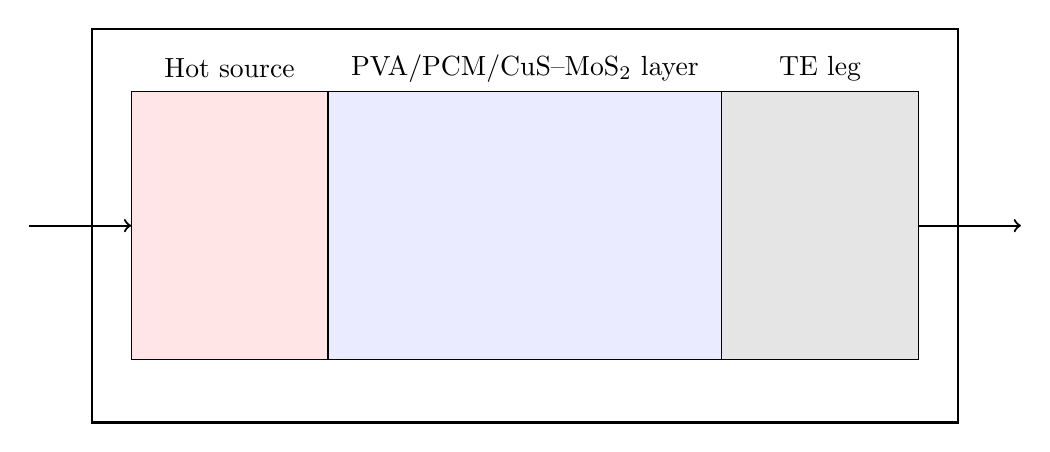
\begin{tikzpicture}
\draw[thick] (0,0) rectangle (11,5);
\draw[fill=red!10] (0.5,0.8) rectangle (3.0,4.2);
\draw[fill=blue!8] (3.0,0.8) rectangle (8.0,4.2);
\draw[fill=gray!20] (8.0,0.8) rectangle (10.5,4.2);
\node at (1.75,4.5) {Hot source};
\node at (5.5,4.5) {PVA/PCM/CuS--MoS$_2$ layer};
\node at (9.25,4.5) {TE leg};
\draw[->,thick] (-0.8,2.5) -- (0.5,2.5);
\draw[->,thick] (10.5,2.5) -- (11.8,2.5);
\end{tikzpicture}
\caption{One-dimensional surrogate arrangement used for coupled PDE simulations.}
\label{fig:multi_domain}
\end{figure}

\begin{table}[htbp]
\centering
\caption{Boundary conditions used in the coupled model.}
\label{tab:multi_bc}
\begin{tabular}{lll}
\toprule
Boundary & Thermal condition & Electrical condition \\
\midrule
Hot side & Prescribed $q''_{in}(t)$ & Insulated \\
Cold side & Convective cooling & Load potential $V_L$ \\
Side walls & Adiabatic & Insulated \\
Interfaces & Kapitza jump & Current continuity \\
\bottomrule
\end{tabular}
\end{table}
